La librería \emph{zapper} provee funcionalidad para buscar y reproducir canales de televisión.

La búsqueda de canales se realiza mediante la clase \hyperlink{classzapper_1_1Tuner}{\texttt{Tuner}}. Por cada canal encontrado se crea una instancia de la clase \hyperlink{classzapper_1_1channel_1_1Channel}{\texttt{Channel}} que almacena información del canal (nombre, descripción, clasificación parental, etc).

La reproducción de canales se realiza mediante la clase \hyperlink{classzapper_1_1MediaPlayer}{\texttt{MediaPlayer}}.

La funcionalidad provista por la librería es expuesta a través de servicios, éstos son accesibles mediante el objeto \hyperlink{classzapper_1_1PluginManager}{\texttt{PluginManager}} que es creado al momento de instanciar la clase \hyperlink{classzapper_1_1Zapper}{\texttt{Zapper}}.

\begin{figure}[h!]
	\centering
	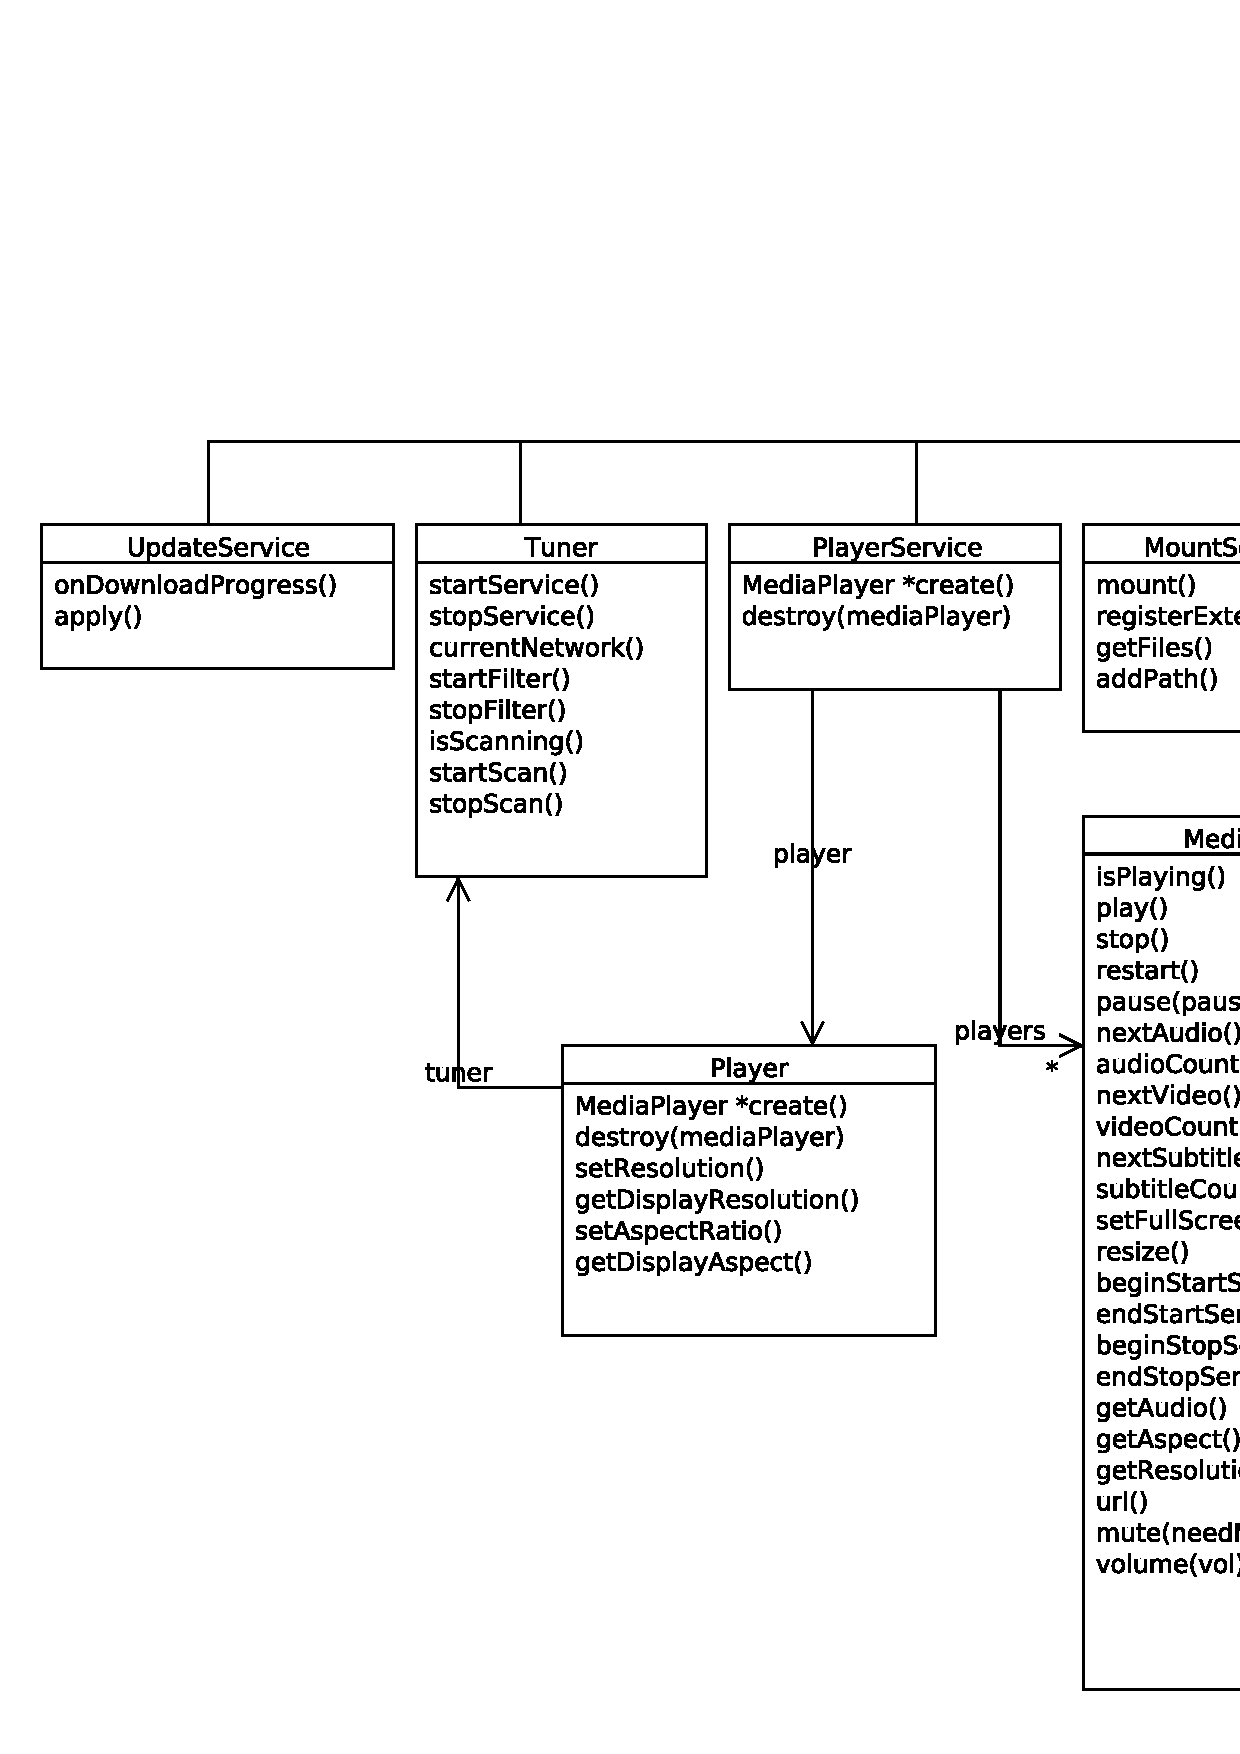
\includegraphics[scale=0.26]{resources/uml-dtv-zapper.jpg}
	\caption{Diagrama de clases de la librería \emph{zapper}.}
\end{figure}
\FloatBarrier

\section{APIs}
La arquitectura de la plataforma define una serie de APIs que agrupan funcionalidad lógicamente relacionada y que definen su comportamiento y alcance. Cada API está compuesta por un conjunto de clases que implementan funcionalidad genérica y definen un protocolo. Para obtener una API funcional es necesario subclasificar éstas clases, implementando el comportamiento faltante. Debemos notar que la mayor parte de las funcionalidades de estas APIs son un 
% TODO: buscar una mejor palabra
\textit{wrapping} 
% ENDTODO: buscar una mejor palabra
de las funcionalidades provistas por la librería \texttt{canvas}.

\subsection{API Input}
Provee funcionalidad que permite la captura y tratamiento de eventos del usuario, como por ejemplo, la pulsación de una tecla. La API está expuesta a través de la clase \textit{canvas::Input}. Actualmente se encuentran subclasificaciones que utilizan las librerías: \textit{LiRC}, \textit{Linux events}, y las provistas por los distintos \textit{Systems} de la librería \textit{canvas} (\textit{GTK}, \textit{DirectFB} y \textit{X11}).

\subsection{API Window}
Provee funcionalidad para la creación, configuración y manipulación de la ventana de la aplicación. El manejo de las ventanas se encuentra dividido en dos partes.

La primera tiene como base a \texttt{zapper::display::DisplayService}, y es responsable de seleccionar conectores (Video Compuesto, por Componentes, HDMI, etc.), la resolución y relación de aspecto de dichos conectores.

La segunda tiene como base a \texttt{canvas::Windows}, su función es la de minimizar, maximizar o cambiar de tamaño la ventana del sistema. Actualmente hay implementaciones de esta parte de la API utilizando las librerías \textit{GTK}, \textit{DirectFB} y \textit{X11}.

\subsection{API Canvas}
Brinda operaciones básicas de dibujo 2D, por ejemplo dibujo de rectángulos, líneas o  composición de imágenes. 

La clase abstracta \textit{canvas::Surface} representa una superficie 2D y es donde se definen todas las primitivas de dibujo. 

Por otro lado, existe la clase \textit{canvas::Canvas} que representa al conjunto de superficies y define la API para la composición y renderizado de las mismas; parte de la responsabilidad de \textit{canvas::Canvas} es la de crear las \textit{canvas::Surfaces}, la forma de crear estas superficies depende de cada implementación y por tanto ésta clase, junto a \textit{canvas::Surface}, debe ser subclasificada. Actualmente hay subclasificaciones que utilizan las librerías: \textit{Cairo(GTK)}, \textit{OpenGL} y \textit{DirectFB}.

\subsection{API WebView}
Provee la funcionalidad necesaria para el renderizado de contenido html a partir de una \textit{URI}. La API está definida en la clase abstracta \textit{canvas::WebViewer}. En este momento hay subclasificaciones utilizando las librerías: \textit{CEF} y \textit{Webkit(GTK)}.

\subsection{Transport Stream Provider}
Esta API es la encargada de obtener información de los Transport Streams, ya sean secciones (PAT, PMT, NIT, etc), o packetized elementary stream (PES: audio, video, close caption, etc); esto se realiza a través de la jerarquía \texttt{Provider}.

La responsabilidad de \texttt{Provider} es la administración de filtros (creación, destrucción, inicio, fin). Estos filtros son representados por la jerarquía \texttt{Filter}, y su función es la de alimentar, con los datos obtenidos, a los distintos componentes que lo requieran. 

Actualmente se encuentra una subclasificación de esta API utilizando la librería \textit{DVB for linux}. También existe una subclasificación a partir de la clase \texttt{TSProvider}, la cual realiza un procesamiento completo del Transport Stream, alimentándose de distintas fuentes (archivos, red, etc).

\subsection{API MediaPlayer}
Provee la funcionalidad necesaria para la decodificación y reproducción de elementos de audio y video. Esta API está expuesta a través de dos clases, la primera es \textit{zapper::MediaPlayer} la cual brinda la interfaz para la reproducción de un elemento de audio o video; la segunda es \textit{zapper::Player}, que define el protocolo para la inicialización de la implementación y la creación de instancias de la clase \textit{zapper::MediaPlayer}.
Además esta API tiene una subclasificación que utiliza la librería \textit{VLC} a través de \textit{canvas::MediaPlayer}.

\subsection{API Mixer}
Las funciones de esta API se utilizan para el control de la salida audio, permitiendo por ejemplo subir/bajar el volumen o poner en estado mute. Esta API está expuesta a través de la clase \textit{zapper::audio::Mixer}.
Esta API posee una subclasificación que utiliza la librería \textit{PulseAudio}.

